\documentclass[letterpaper]{article}

\title{Reading 08: Document Tools}
\date{Monday March 14, 2016}
\author{Michael McRoskey}

\usepackage{graphicx}
\usepackage{hyperref}
\usepackage[margin=1in]{geometry}

\begin{document}

\maketitle

%------------------------------------------------------------------------------

\section*{Overview}

For this experiement, I created {\bf two} scripts, {\bf one} gnu plot file, and a makefile

\begin{itemize} 
   \item \textbf{roll\_dice.sh} : This script simulates rolling a dice.
   \item \textbf{experiment.sh} : This script uses \texttt{roll\_dice.sh} to perform an experiment and then collect that data
into \texttt{results.dat}.
   \item \textbf{histogram.plt} :  This script uses gnuplot to create a graph of the data in texttt{results.dat}.
 \end{itemize}

%------------------------------------------------------------------------------

\section*{Rolling Dice}

The first script \texttt{roll\_dice.sh} uses a while getopts loop to take in extra parameters and otherwise executes a simple for loop with the \texttt{shuf} command within the range of 1-6.

\begin{verbatim}
usage: roll_dice.sh [-r ROLLS -s sides]

	    -r ROLLS        Number of rolls of die (default: 10)
	    -s SIDES        Number of sides on die (default: 6)
\end{verbatim}


%------------------------------------------------------------------------------

\section*{Experiment}

The experiment script simulates 1000 rolls by:
\begin{itemize}
	\item Calling \texttt{roll\_dice.sh} with r=1000 rolls
	\item Using \texttt{awk} to determine the number of samples of the randomly generated number
	\item Using \texttt{sort} to show the output for 1, 2, 3, 4, 5 and 6
	\item Output results using \texttt{awk} to a tsv file
\end{itemize}

%------------------------------------------------------------------------------

\section*{Results}

Table 1 contains the results of my experiment of rolling a dice 1000 times:

\begin{table}[h!]
	\centering
	\begin{tabular}{c|c}
	Side & Counts\\
	\hline
	1 & 195\\
	2 & 163\\
	3 & 142\\
	4 & 159\\
	5 & 173\\
	6 & 168\\
	\end{tabular}
	\caption{Dice Rolling Results}
	\label{tbl:results}
\end{table}

Figure 1 contains a plot of my experimental results as produced by \texttt{histogram.plt}:

\begin{figure}[h!]
	\centering
	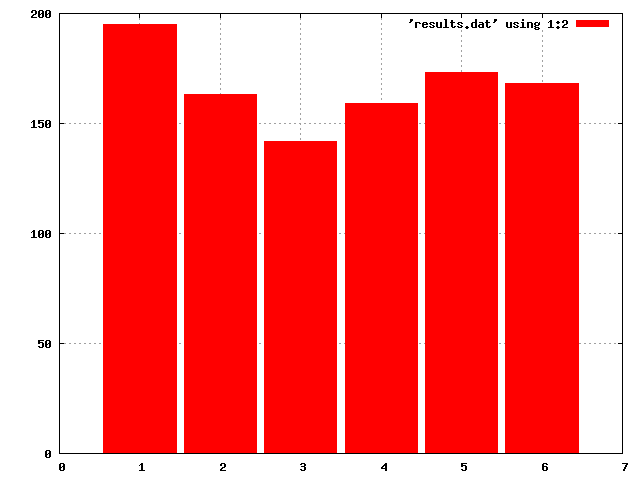
\includegraphics[width=5in]{results.png}
	\caption{Dice Rolling Results}
	\label{fig:results}
\end{figure}

\end{document}

